% Chapter Template

\chapter{SIMULACIONES ATOMISTICAS} % Main chapter title

\label{C2} % Change X to a consecutive number; for referencing this chapter elsewhere, use {ChapterX}

\lhead{Capítulo 2. \emph{SIMULACIONES ATOMISTICAS}} % Change X to a consecutive number; this is for the header on each page - perhaps a shortened title

%----------------------------------------------------------------------------------------
%	SECTION 1
%----------------------------------------------------------------------------------------

\section{Simulación, Teoría y Experimentos}
\label{S2_1}

Las simulaciones en computadora han abierto la posibilidad a estudiar sistemas, y verificar modelos bajo condiciones que son imposibles (o muy difíciles) de conseguir experimentalmente. También han permitido incrementar la complejidad de los modelos usados y realizar comparaciones directas con fenómenos naturales, una vez que el modelo ha sido validado.

Con la llegada de computadoras más potentes, aparece una nueva opción a considerar entre teoría y experimentos: los experimentos numéricamente simulados. El modelo sobre el cual se realiza esta simulación sigue siendo teórico, pero todos los cálculos son llevados a cabo por la computadora. Es muy importante por supuesto, definir las condiciones de simulación de tal manera que represente una situación físicamente posible, y no obtener resultados absurdos. Para ello, los modelos teóricos y numéricos son previamente calibrados mediante los resultados obtenidos de experimentos.

Tanto el modelo como las condiciones de simulación y los elementos que componen el experimento simulado se encuentran en el marco de algún paquete de software que mediante algoritmos específicos resuelven el problema y nos entregan ciertos resultados.

En este trabajo en particular se hace uso de simulaciones de Dinámica Molecular (apropiadas para estudiar fenómenos en escala nano) mediante el paquete LAMMPS \citep{plimpton95}, que es de código abierto y gratuito.

%----------------------------------------------------------------------------------------
%	SECTION 2
%----------------------------------------------------------------------------------------

\section{Introducción a Dinámica Molecular}
\label{S2_2}

Las simulaciones de dinámica molecular (MD) son usadas frecuentemente para estudiar propiedades a escala nano \citep{allen87}. Las simulaciones de MD son una técnica muy poderosa que permite resolver, usando mecánica clásica, problemas con muchos cuerpos, dada una interacción entre átomos. Una ventaja de MD es que la deformación, el esfuerzo, la temperatura, la velocidad, etc. son todas conocidas en detalle \citep{allen87}. Con esta información un gran número de fenómenos pueden estudiarse, como cambios de fase, transferencia de calor, creación y movimiento de dislocaciones, defectos, etc.. MD es una herramienta muy versátil para el estudio de las propiedades de materiales, y hasta ha sido utilizada para predecir el comportamiento mecánico de materiales previamente a los experimentos, como en el caso de maclas de aluminio \citep{chen03}. Las simulaciones de MD reproducen el movimiento atómico y por lo tanto emplean pasos de tiempo de 1 fs \citep{allen87}.

Las simulaciones de MD integran en el tiempo las ecuaciones de movimiento de Newton para un grupo de $N$ átomos, dadas por:

\begin{equation}
\mathbf{F_{i}} = m_{i}\mathbf{a_{i}}
\end{equation}

donde $m_{i}$ es la masa de cada átomo y $\mathbf{a_{i}}$ es su aceleración, dada por $\frac{d^{2}\mathbf{r_{i}}}{dt^{2}}$. De lo anterior se puede concluir lo siguiente:

\begin{itemize}
 \item El resultado final de dos simulaciones de MD para iguales condiciones iniciales producen, en teoría, los mismos resultados, es decir, son deterministas (los errores de redondeo propios del cálculo numérico hacen que las soluciones diverjan de todas maneras).
 \item Si el número de átomos es pequeño, dos condiciones iniciales ligeramente distintas pueden llevar a soluciones muy diferentes.
 \item En sistemas con un gran número de átomos las soluciones para distintas condiciones iniciales deberían ser estadísticamente similares (los estados termodinámicos son comparables).
\end{itemize}

El estado termodinámico del sistema está definido por ciertos parámetros como la temperatura, la presión, el número de partículas, etc. El estado microscópico del sistema queda definido por las posiciones $p_{i}$ y los momentos atómicos $q_{i}$ y lo llamamos \textbf{espacio de fase}. Las posiciones y los momentos son considerados coordenadas de un espacio $6N$-dimensional ($\Omega$), en el que un punto cualquiera se denomina $P$ y describe el estado del sistema. 

Todas las configuraciones posibles que tienen diferente estado microscópico pero tienen idéntico estado macroscópico o termodinámico se denomina \textbf{ensamble estadístico}. En una simulación de MD, se aplican restricciones o condiciones externas, que determinan el tipo de ensamble, es decir, las sucesivos valores de velocidad y posición que obtenemos en cada paso de la simulación son configuraciones diferentes del mismo ensamble.

Las propiedades termodinámicas se calculan como promedios de ciertas funciones que aplican sobre la configuración del sistema (un \textbf{observable} $\mathbf{\mathcal{A}}(p_{i},q_{i})$) sobre todas las configuraciones posibles:

\begin{equation}
\langle \mathbf{\mathcal{A}} \rangle _{ens}
\end{equation}

Esto resulta extremadamente difícil dado el número enorme de configuraciones posibles. Otra forma de calcular el promedio de este observable es considerar el promedio en el tiempo del mismo. Dicho de otro modo, considerando que los puntos $P_{i}$ de salida de la simulación forman una trayectoria $\mathbf{\Gamma}(t)$ en el espacio de fase, puede calcularse el promedio en el tiempo, como una función de $\mathbf{\Gamma}(t)$:

\begin{equation}
\langle \mathbf{\mathcal{A}} \rangle _{t} = \frac{1}{\tau_{obs}} \sum_{\tau = 1}^{\tau_{obs}} \mathbf{\mathcal{A}}(\Gamma (t))
\end{equation}

donde $\tau$ representa un paso de simulación y $\tau_{obs}$ es el número total de pasos.

Si bien estos dos promedios se definen de diferente manera, la \textbf{hipótesis ergódica} nos dice que los dos son iguales. Definimos un sistema \textbf{ergódico} como un sistema para el cual, sobre un conjunto $V$ de $\Omega$, el Promedio de Tiempo\footnotemark[1] de una función $\mathbf{\mathcal{A}}$ a lo largo de una trayectoria $\mathbf{\Gamma}(t)$ es igual al Promedio de Fase\footnotemark[2] de $\mathbf{\mathcal{A}}$ en casi todas partes\footnotemark[3].

\footnotetext[1]{$\lim_{t\to\infty} \int_{0}^{t} \mathbf{\mathcal{A}}(P,T) dt = \bar{\mathbf{\mathcal{A}}}(P)$ se llama Promedio de Tiempo de $\mathbf{\mathcal{A}}$ a lo largo de la trayectoria que pasa por $P$}
\footnotetext[2]{El teorema de Birkhoff dice: Sea $V$ un subconjunto del Espacio de Fase $\Omega$ invariante bajo una trasformación $T:V\rightarrow{}V$ y que tiene un volumen generalizado finito. Sea  $\mathbf{\mathcal{A}}$ =  $\mathbf{\mathcal{A}}(P)$, una función de fase, definida para todos los puntos de $V$ e integrable sobre $V$. Entonces el límite $\lim_{t\to\infty} \int_{0}^{t} \mathbf{\mathcal{A}}(P,T) dt$ existe para casi todos los puntos de $V$}
\footnotetext[3]{$\frac{1}{\mu{}(V)} \int_{V} \mathbf{\mathcal{A}}(p) dV$ se llama Promedio de Fase de $\mathbf{\mathcal{A}}$ sobre $V$ y es el promedio de la función $\mathbf{\mathcal{A}}$, calculado sobre el conjunto invariante $V$}

Esto quiere decir que podemos calcular propiedades termodinámicas a partir del Promedio de Tiempo de la propiedad de interés, sin tener que calcular el promedio del ensamble. La idea es que con tiempos suficientemente grandes, el sistema pasa por un número de estados suficientemente grande para considerar estos dos promedios iguales:

\begin{equation}
\langle \mathbf{\mathcal{A}} \rangle _{t} = \langle \mathbf{\mathcal{A}} \rangle _{ens}
\end{equation}

Existen diferentes ensambles, como por ejemplo:

\begin{itemize}
	\item \textbf{Ensamble Microcanónico $(N,V,E)$}: Se fija el número de partículas, el volumen y la energía total.
	\item \textbf{Ensamble Canónico $(N,V,T)$}: Se fija el número de partículas, el volumen y la temperatura.
	\item \textbf{Ensamble Macrocanónico $(\mu,V,T)$}: Se fija el potencial químico, el volumen y la temperatura.
	\item \textbf{Ensamble Isotérmico-Isobárico $(N,P,T)$}: Se fija el número de partículas, la presión y la temperatura.
	\item \textbf{Ensamble Isobárico-Isoentálpico $(N,P,H)$}: Se fija el número de partículas, la presión y la entalpía.
\end{itemize}

%----------------------------------------------------------------------------------------
%	SECTION 3
%----------------------------------------------------------------------------------------
\section{Potenciales Interatómicos}
\label{S2_3}

El grado de semejanza a la realidad que puede tener una simulación de MD depende (entre otros) de que las fuerzas interatómicas simuladas representen las presentes en el material real. Estas fuerzas son calculadas internamente como el gradiente de una \textit{función de energía potencial}, que depende de las posiciones atómicas (Ecuaciones \ref{C2:eq:pot} y \ref{C2:eq:potfza}). Hay que aclarar que esta función puede responder bien a determinadas condiciones o composiciones, pero no a otras: hay que estar seguro de que el potencial es representativo para las condiciones de nuestra simulación.
\vspace{-0.3pt}
\begin{align}
& V(\mathbf{r}_{1},...,\mathbf{r}_{2})
\label{C2:eq:pot}\\
\mathbf{F}_{i} = & -\nabla_{\mathbf{r}_{i}}V(\mathbf{r}_{1},...,\mathbf{r}_{2})
\label{C2:eq:potfza}
\end{align}

Existen numerosos potenciales utilizados actualmente, algunos más generales que otros y con diferente formulación. Para sistemas complejos, los potenciales se generan en forma tabular, y no se tiene una expresión analítica del mismo, debiendo usarse el que corresponda a nuestra composición y parámetros de simulación.

Se nombran dos ejemplos a continuación: el potencial \textit{Lennard-Jones} y el \textit{Modelo de Átomo Embebido (EAM)}. El último es el que se utiliza en todas las simulaciones de MD del presente trabajo.

\subsection{Potencial Lennard-Jones}
\label{SS2_3_1}

El potencial Lennard-Jones es un modelo simple que describe la interacción entre dos átomos neutrales, y su expresión matemática se ve en la \eref{eq:LJ}. El valor $\gamma$ es la profundidad del pozo de energía potencial, $r_{0}$ es la distancia a la cual el potencial es cero, $r_{m}$ es la distancia para la cual se obtiene el mínimo de energía potencial y $r$ es la distancia entre los átomos. A $r_{m}$, el potencial vale $-\gamma$.

\begin{equation}
V_{LJ}=4\gamma \left[ \left( \frac{r_{0}}{r} \right)^{12} - \left( \frac{r_{0}}{r} \right)^{6} \right] = 
\gamma \left[ \left( \frac{r_{m}}{r} \right)^{12} -2 \left( \frac{r_{m}}{r} \right)^{6} \right]
\label{eq:LJ}
\end{equation}

El término con $r^{-12}$ es un término de repulsión asociado a la repulsión de Pauli\footnotemark[4] y el término con $r^{-6}$ representa la atracción de largo alcance (fuerzas de van der Waals\footnotemark[5]). Podemos ver gráficamente el potencial en la \fref{C2:fg:LJ}.

\footnotetext[4]{Esta contribución repulsiva proviene del recubrimiento parcial entre orbitales atómicos}
\footnotetext[5]{Las fuerzas de van der Waals están asociadas a la atracción interatómica debida a los momentos dipolares.}

\begin{figure}[htp]
\centering
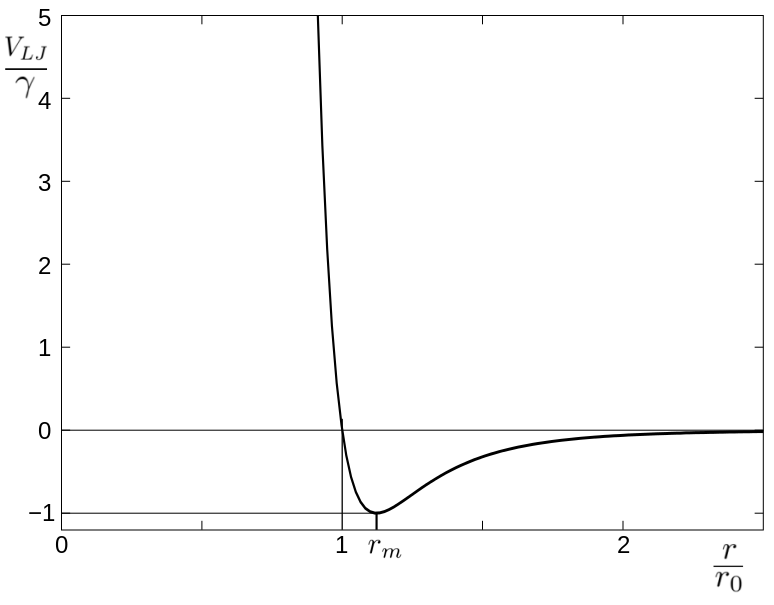
\includegraphics[width=10cm]{Cap_2/LJ.png}
\caption[Potencial de Lennard-Jones]{Gráfica del potencial Lennard-Jones normalizado a $\gamma$ y $r_{0}$}
\label{C2:fg:LJ}
\end{figure}

\subsection{Modelo de Átomo Embebido}
\label{SS2_3_2}

Este modelo es descrito en detalle en el trabajo de \cite{daw84}. En el mismo, la energía potencial es función de una suma de funciones de la separación entre un átomo y sus vecinos. La energía potencial de un átomo $i$ está dada por la \eref{C2:eq:EAM}:

\begin{equation}
V_{i} = F_{\alpha}\left(\sum_{i\neq j} \rho_{\beta} (r_{ij}) \right) + \frac{1}{2} \sum_{i\neq j} \phi_{\alpha\beta}(r_{ij})
\label{C2:eq:EAM}
\end{equation}

donde $r_{ij}$ es la distancia entre los átomos $i$ y $j$, $\phi_{\alpha\beta}$ es una función potencial entre pares de átomos, $\rho_{\beta}$ es la contribución a la densidad de carga electrónica del átomo $j$ de tipo $\beta$ en la ubicación del átomo $i$ y $F_{\alpha}$ es una función que representa la energía requerida para colocar el átomo $i$ de tipo $\alpha$ en la nube de electrones.

Al definir las funciones $\phi_{\alpha\beta}(r_{ij})$, $F_{\alpha}(\rho)$ y $\rho_{\beta} (r_{ij})$ se establece el modelo para un material en particular. En el caso de nuestras simulaciones, se tiene una aleación metálica de dos componentes, lo que implica definir siete funciones: tres funciones potenciales ($\phi_{\alpha\alpha}$, $\phi_{\alpha\beta}$, $\phi_{\beta\beta}$), dos funciones integradoras ($F_{\alpha}$, $F_{\beta}$) y dos funciones de contribución a la densidad de carga electrónica ($\rho_{\alpha}$, $\rho_{\beta}$).

Las funciones se encuentran en forma tabular en un archivo de formato \textit{setfl} \citep{setfl} que es leído por LAMMPS al indicarlo en el script de entrada. El archivo que utilizamos en nuestras simulaciones fue realizado por H.W.Sheng \citep{cheng09}.

%----------------------------------------------------------------------------------------
%	SECTION 4
%----------------------------------------------------------------------------------------
\section{Integración de las Ecuaciones de Movimiento}
\label{S2_4}

Existen diferentes algoritmos para la resolución numérica de las ecuaciones de movimiento de las partículas simuladas. En general, todos los métodos parten de la expansión en serie de Taylor de la posición y velocidad en función del tiempo. Esto, junto con la implementación computacional del algoritmo, hacen que siempre estén presentes dos errores: un error de truncamiento de la expansión en serie de Taylor, y un error de redondeo al usar un número finito de posiciones decimales.

Si bien los dos errores son inevitables, el error de truncamiento es propio del algoritmo y no podemos cambiar \textit{su orden}, mientras que el error de redondeo varía según la manera en que se haya implementado las operaciones matemáticas a nivel informático. Para $\Delta{}t$ grandes, predomina el error de truncamiento, mientras que para $\Delta{}t$ tendiendo a cero, predominan los errores de redondeo.

En este apartado describiremos los métodos \textbf{Verlet} (Sección \ref{S2_4_1}) y \textbf{Velocity Verlet} (Sección \ref{S2_4_2}). Este último es el usado por LAMMPS para nuestras simulaciones.

\subsection{Integración Verlet}
\label{S2_4_1}

Expandimos en primer lugar en serie de Taylor la posición para $t+\Delta{}t$ y $t-\Delta{}t$:
\vspace{-0.3pt}
\begin{align}
\mathbf{r}(t+\Delta{}t) & = \mathbf{r}(t)+\frac{d\mathbf{r}(t)}{dt} \Delta{}t + \frac{1}{2} \frac{d^{2}\mathbf{r}(t)}{dt^{2}} \Delta{}t^{2} + \frac{1}{3!} \frac{d^{3}\mathbf{r}(t)}{dt^{3}} \Delta{}t^{3} + \mathcal{O}(\Delta{}t^{4})
\label{C2:eq:VerletTaylor1} \\
\mathbf{r}(t-\Delta{}t) & = \mathbf{r}(t)-\frac{d\mathbf{r}(t)}{dt} \Delta{}t + \frac{1}{2} \frac{d^{2}\mathbf{r}(t)}{dt^{2}} \Delta{}t^{2} - \frac{1}{3!} \frac{d^{3}\mathbf{r}(t)}{dt^{3}} \Delta{}t^{3} + \mathcal{O}(\Delta{}t^{4})
\label{C2:eq:VerletTaylor2}
\end{align}

Sumando las Ecuaciones \ref{C2:eq:VerletTaylor1} y \ref{C2:eq:VerletTaylor2} y restando $\mathbf{r}(t-\Delta{}t)$ en ambos miembros obtenemos:

\begin{equation}
\mathbf{r}(t+\Delta{}t) = 2\mathbf{r}(t) - \mathbf{r}(t-\Delta{}t) + \frac{d^{2}\mathbf{r}(t)}{dt^{2}} \Delta{}t^{2} + \mathcal{O}(t^{4})
\label{C2:eq:VerletPos}
\end{equation}

La aceleración es calculada mediante el potencial visto anteriormente (\eref{C2:eq:potfza}) como:

\begin{equation}
\mathbf{a}(t) = \frac{d^{2}\mathbf{r}(t)}{dt^{2}} = -\frac{1}{m}\nabla{}V(\mathbf{r}(t))
\end{equation}

Una desventaja de este método es que las velocidades no se calculan directamente, y en general se obtienen de una aproximación por diferencias finitas centrales según:

\begin{equation}
\mathbf{v}(t) = \frac{\mathbf{r}(t+\Delta{}t) - \mathbf{r}(t-\Delta{}t)}{2\Delta{}t} + \mathcal{O}(t^{2})
\end{equation}

con lo cual el error deja de ser de $\mathcal{O}(\Delta{}t^{4})$ para ser de $\mathcal{O}(\Delta{}t^{2})$. Otro inconveniente es que para calcular las posiciones en un paso de tiempo, son necesarias las posiciones de dos pasos de tiempo atrás, por lo que el algoritmo requiere una inicialización de dos pasos. Esto último se resuelve en el método que se describe en el siguiente apartado.

\subsection{Integración Velocity Verlet}
\label{S2_4_2}

Partimos de la expansión en serie de Taylor de la posición y la velocidad en $t+\Delta{}t$:
\vspace{-0.3pt}
\begin{align}
\mathbf{r}(t+\Delta{}t) & = \mathbf{r}(t)+\frac{d\mathbf{r}(t)}{dt} \Delta{}t + \frac{1}{2} \frac{d^{2}\mathbf{r}(t)}{dt^{2}} \Delta{}t^{2} + \mathcal{O}(\Delta{}t^{3})
\label{C2:eq:VelVerletTaylor1} \\
\mathbf{v}(t+\Delta{}t) & = \mathbf{v}(t)+\mathbf{a}(t)\Delta{}t + \frac{1}{2}\frac{d\mathbf{a}(t)}{dt} \Delta{}t^{2} + \mathcal{O}(\Delta{}t^{3})
\label{C2:eq:VelVerletTaylor2}
\end{align}

La \eref{C2:eq:VelVerletTaylor2} puede reescribirse partiendo de la expansión en serie de Taylor de la aceleración:
\vspace{-0.3pt}
\begin{align}
\mathbf{a}(t+\Delta{}t) & = \mathbf{a}(t)+\frac{d\mathbf{a}(t)}{dt} \Delta{}t + \mathcal{O}(\Delta{}t^{2})
\label{C2:eq:tayloracc1} \\
\mathbf{a}(t)+\mathbf{a}(t+\Delta{}t) & = 2\mathbf{a}(t)+\frac{d\mathbf{a}(t)}{dt} \Delta{}t + \mathcal{O}(\Delta{}t^{2})
\label{C2:eq:tayloracc2} \\
\frac{1}{2}\Delta{}t\left[\mathbf{a}(t)+\mathbf{a}(t+\Delta{}t)\right] & = \mathbf{a}(t)\Delta{}t+\frac{1}{2}\frac{d\mathbf{a}(t)}{dt} \Delta{}t^{2} + \mathcal{O}(\Delta{}t^{3})
\label{C2:eq:tayloracc3}
\end{align}

Introduciendo la \eref{C2:eq:tayloracc3} en la \eref{C2:eq:VelVerletTaylor2}, obtenemos:

\begin{equation}
\mathbf{v}(t+\Delta{}t) = \mathbf{v}(t)+\frac{1}{2}\Delta{}t\left[\mathbf{a}(t)+\mathbf{a}(t+\Delta{}t)\right] + \mathcal{O}(\Delta{}t^{3})
\label{C2:eq:VelVerletTaylor3}
\end{equation}

Ahora podemos realizar la integración siguiendo los pasos a continuación:

\begin{enumerate}
	\item Calcular la velocidad en el paso de tiempo medio $t+\frac{\Delta{}t}{2}$
	\begin{equation}
	\mathbf{v}\left(t+\frac{\Delta{}t}{2}\right) = \mathbf{v}(t) + \frac{1}{2}\mathbf{a}(t)\Delta{}t
	\end{equation}
	\item Calcular las posiciones en el paso de tiempo $\Delta{}t$
	\begin{equation}
	\mathbf{r}(t+\Delta{}t) = \mathbf{r}(t) + \mathbf{v}\left(t+\frac{\Delta{}t}{2}\right)\Delta{}t
	\end{equation}
	\item Calcular las aceleraciones a partir del potencial
	\begin{equation}
	\mathbf{a}(t+\Delta{}t) = -\frac{1}{m}\nabla{}V\left(\mathbf{r}(t+\Delta{}t)\right)
	\end{equation}
	\item Actualizar las velocidades
	\begin{equation}
	\mathbf{v}(t+\Delta{}t) = \mathbf{v}\left(t+\frac{\Delta{}t}{2}\right) + \frac{1}{2}\mathbf{a}\left(t + \Delta{}t\right)\Delta{}t
	\end{equation}
\end{enumerate}

%----------------------------------------------------------------------------------------
%	SECTION 5
%----------------------------------------------------------------------------------------
\section{Termostatos y Barostatos}
\label{S2_5}

Si bien en las simulaciones básicas de MD se utiliza el ensamble microcanónico (NVE), para representar ciertos experimentos se necesita mantener constante otra variable que no sea la energía. Por ejemplo, una reacción química que se realiza en atmósfera libre sucede a presión constante y usamos el ensamble NPT; una reacción biológica puede ocurrir a temperatura constante y usaríamos el ensamble NVT.

Existen diversos métodos para mantener estos parámetros estables:

\begin{itemize}
	\item \textbf{Estocásticos}: Se obliga a una variable del sistema a seguir cierta distribución estadística.
	\item \textbf{De acoplamiento fuerte}: Se aplica una escala a una variable del sistema para llegar al valor exacto de la propiedad derivada.
	\item \textbf{De acoplamiento débil}: Se aplica una escala a una variable del sistema para establecer la tendencia de cambio hacia el valor deseado.
	\item \textbf{De extensión de la dinámica del sistema}: Se agregan grados de libertad adicionales.
\end{itemize}

Se explicará en el apartado siguiente un método usado en nuestras simulaciones para establecer la temperatura deseada mientras se simula con el ensamble NVE.

\subsection{Re-escalado de velocidades}
\label{S2_5_1}
Este método (en inglés \textit{velocity rescaling}) corresponde a un acoplamiento fuerte. Se calcula un factor $\lambda$ que multiplica a todas las velocidades de traslación del sistema. No se escalan las rotaciones. La temperatura del sistema se calcula según:

\begin{equation}
\sum_{i=1}^{N}\frac{m_{i}|\mathbf{v}_{i}|^{2}}{2} = \frac{k_{b}T}{2}(3N-N_{c})
\end{equation}

donde $k_{b}$ es la constante de Boltzmann, $\mathbf{v}_{i}$ las velocidades atómicas lineales, $m_{i}$ las masas atómicas, $T$ la temperatura, $N_{c}$ las restricciones y $3N-N_{c} = N_{gl}$ el número de grados de libertad. Entonces:

\begin{equation}
T = \sum_{i=1}^{N}\frac{m_{i}v_{i}^{2}}{N_{gl}k_{b}}
\end{equation}

Si multiplicamos las velocidades por un factor $\lambda$ para generar un salto $\Delta{}T$, calculamos $\lambda$ como sigue:

\begin{align}
\Delta{}T &= \sum_{i=1}^{N}\frac{m_{i}(\lambda{}v_{i})^{2}}{N_{gl}k_{b}} - \sum_{i=1}^{N}\frac{m_{i}v_{i}^{2}}{N_{gl}k_{b}}\\
T_{\tau} - T_{\tau{}-1} &= (\lambda{}^{2}-1)T_{\tau{}-1}\\
\frac{T_{\tau}}{T_{\tau{}-1}} - 1 &= \lambda{}^{2}-1 \\
\lambda{} &= \sqrt{\frac{T_{\tau{}}}{T_{\tau{}-1}}}
\end{align}

donde $T_{\tau{}-1}$ es la temperatura del paso de tiempo $\tau{}-1$ ya calculado y $T_{\tau}$ es la nueva temperatura.